\documentclass[rep.tex]{subfiles}
\begin{document}

\chapter{Zadanie 7}
\label{zad7}
\section{Treść}
Zaprojektować powietrzne cylindryczno-płaskie linie sprzężone dla następujących danych:
$Z_{0e} = 60~\Omega$, $Z_{0o} = 40~\Omega$.
Obliczenia wykonać przy założeniu,
że odległość pomiędzy dwoma zewnętrznymi płaszczyznami przewodzącymi jest równa~$h = 8~mm$, rys.~\ref{fig:zad7:cf}.

\begin{figure}[!htbp]
  \centering
  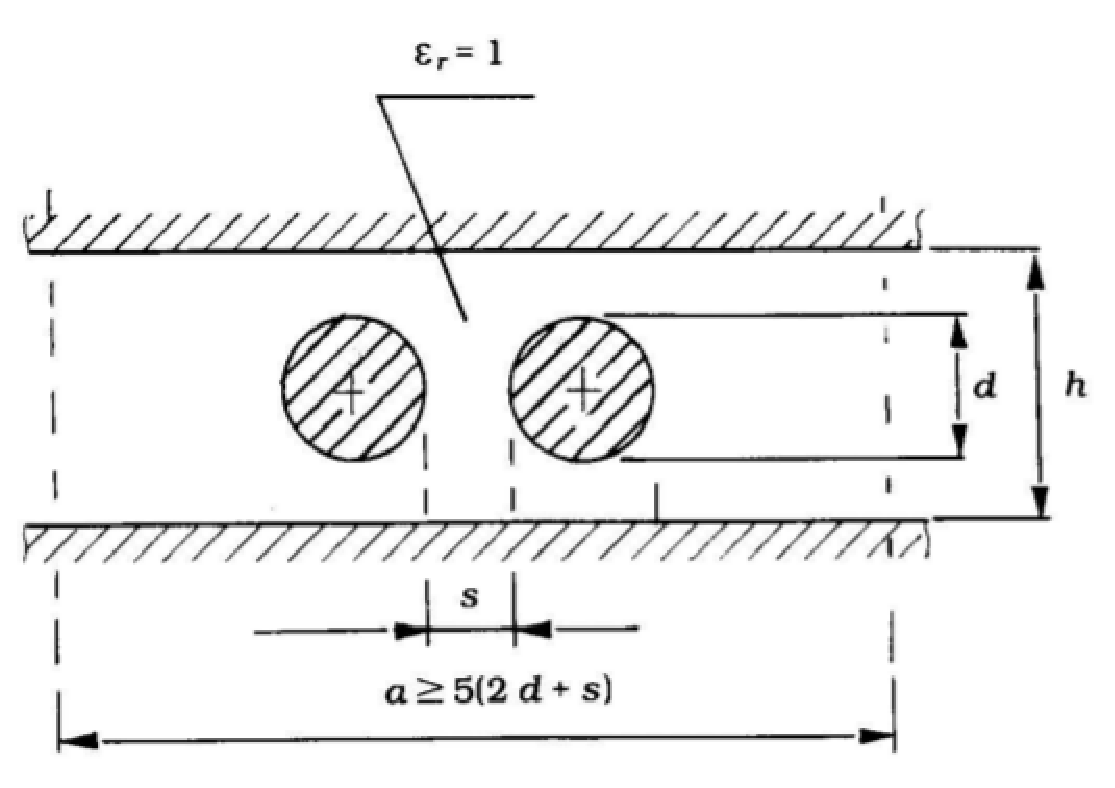
\includegraphics[scale=0.5]{fig/zad7/cf}
  \caption{Lnie cylindryczno-płaskie sprzężone}
  \label{fig:zad7:cf}
\end{figure}

\section{Rozwiązanie}
Impedancje charakterystyczne powietrznych linii cylindryczno-płaskich,
przy pobudzeniu synfazowym~$Z_{0e}$ i przeciwfazowym~$Z_{0o}$ określone są wzorami:
\begin{align}
  Z_{0e}(x, y) &= 59.952 \ln \Bigg( \frac{0.523962}{f_1(x) f_2(x, y) f_3(x, y)} \Bigg) \\
  Z_{0o}(x, y) &= 59.952 \ln \Bigg( \frac{0.523962 f_3(x, y)}{f_1(x) f_4(x, y)} \Bigg)
\end{align}
gdzie:\\
\begin{tabular}{l @{ - } l}
  $f_{(1/2/3/4)}$ & funkcje opisane w~\cite{obwody}, \\
  $x = \frac{d}{h}$ & stosunek średnicy przewodu do odstępu między płaszczyznami, \\
  $y = \frac{s}{h}$ & stosunek odstępu między przewodami do odstępu między płaszczyznami. \\
\end{tabular}

Projektowanie linii sprowadza się do znalezienia takich $x$ i $y$ dla których spełnione są równania:
\begin{align}
  V1(x, y) &= Z_{0e}(x, y) - Z_{0e} = 0 \\
  V2(x, y) &= Z_{0o}(x, y) - Z_{0o} = 0
\end{align}
a finalnie $s$ i $d$.

Implementując metodę Newtona linia spełniająca wymagania postawione w treści zadania ma wymiary: $s = 1.97191812203~mm$ i $d = 4.25688390818~mm$.
\end{document}
